\documentclass[a4paper]{article}

\usepackage[english]{babel}
\usepackage[utf8]{inputenc}
\usepackage{amsmath}
\usepackage{graphicx}
\usepackage[colorinlistoftodos]{todonotes}

\title{Map Matching of Outdoor Trajectory using Hidden Markov Model}

\author{Imam Mustafa Kamal (201683609) &
Nur Ahmad Wahid (201799145)}

\date{\today}

\begin{document}
\maketitle

\section{Introduction}
\label{sec:introduction}

Map Matching problem is the problem of how to match recorded geographic coordinates to a logical model of the real world. The most obvious algorithm is to simply match each point with the nearest road. Due to measurement noise, however, this algorithm is prone to error. Therefore, a more powerful and more reliable method is needed. The paper mentioned in the title of our proposal implement Hidden Markov Model that elegantly accounts for measurement noise and the layout of the road network.

GraphHopper Routing Engine is a fast and memory efficient Java routing engine open source presented by Graphhopper company that focuses on providing routing services. OpenStreetMap (OSM) is a collaborative project to create a free editable map of the world. Rather than the map itself, the data generated by the project is considered its primary output. The creation and growth of OSM has been motivated by restrictions on use or availability of map information across much of the world, and the advent of inexpensive portable satellite navigation devices.

Nowadays, the trajectory data is extremely large. Many trajectory data are generated from taxi, mobile phone, and other smart devices. However, due to the average error rate of Global Positioning Systems (GPS) in tracking object is not less than 10\% Therefore, the generated trajectory data commonly is not accurate and tend to be noisy. The trajectory that generated by moving object sometimes far from the appropriate road network, due to GPS error, and using high sampling rate. Currently, map matching is becoming important as vehicles are used as traffic monitoring and route prediction, and activity recognition. Therefore, we conducted a study for map-matching vehicle trajectory against the road network.


\section{Problem}
\label{sec:problem}

Map matching can be implemented on either offline data trajectory like this experiment conducted, or online/real time trajectory data like demonstrated by the paper Eddy: An Error-bounded Delay-bounded real-time map matching using HMM and online Viterbi Decoder [4]. Not only by using HMM, map matching can also be done by using another technique such as Reinforcement Learning like shown by Takayuki Osogami and Rudy Raymond [5].

In this study, we conducted experiment on basic problem in map matching with offline data using HMM.
The straight-forward way to solve map-matching issue is map the vehicle location to the near road network. Due to the GPS error and other factor that makes the trajectory data to be noisy, this mechanism incurs a problem if the vehicle is located in near many road network as illustrated in figure 1.

\begin{figure}
\centering
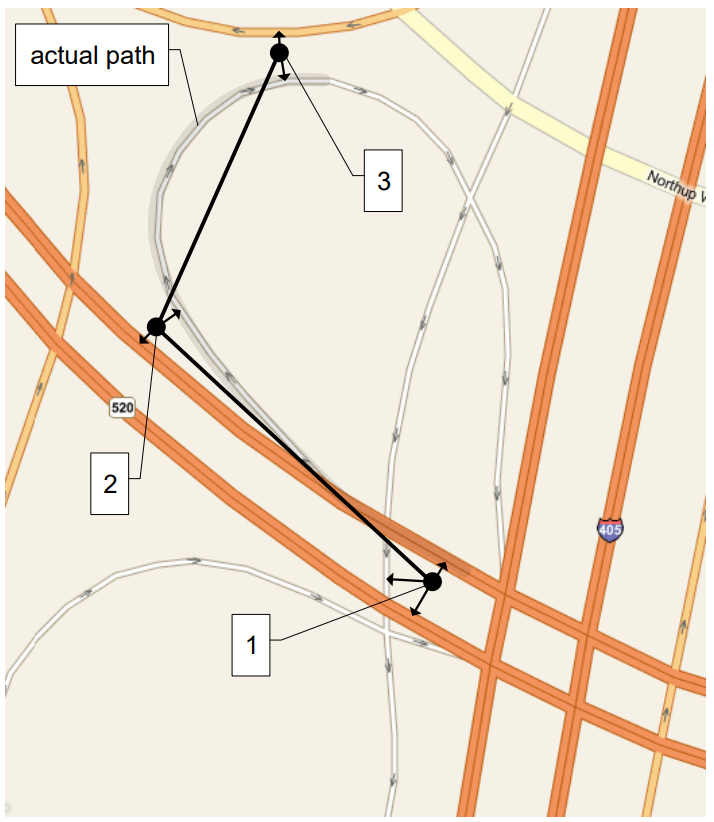
\includegraphics[width=0.5\textwidth]{fig1.png}
\caption{\label{fig:data} Map matching issue in many road networks [1]}
\end{figure}

\section{Proposed Method}
\label{sec:method}

To do map matching, we conduct a study for matching trajectory data to road network using Hidden Markov Model (HMM). The input is a tuple of time-stamped with latitude/longitude. The roads are also represented in the traditional way, as a graph representation, wherein it consists of nodes and edges. The nodes are able to represent as an intersection, a dead end road, or a road name changes, and the edges corresponds road segments between the nodes. The Hidden Markov Model representation is depicted in figure 2. The state is road segment, in this research, it is denoted as $r$. Where the set of road segments ($r$) candidate are derived from GaphHopper API, while t represents the particular time of object is located by detecting the longitude and latitude.

\begin{figure}
\centering
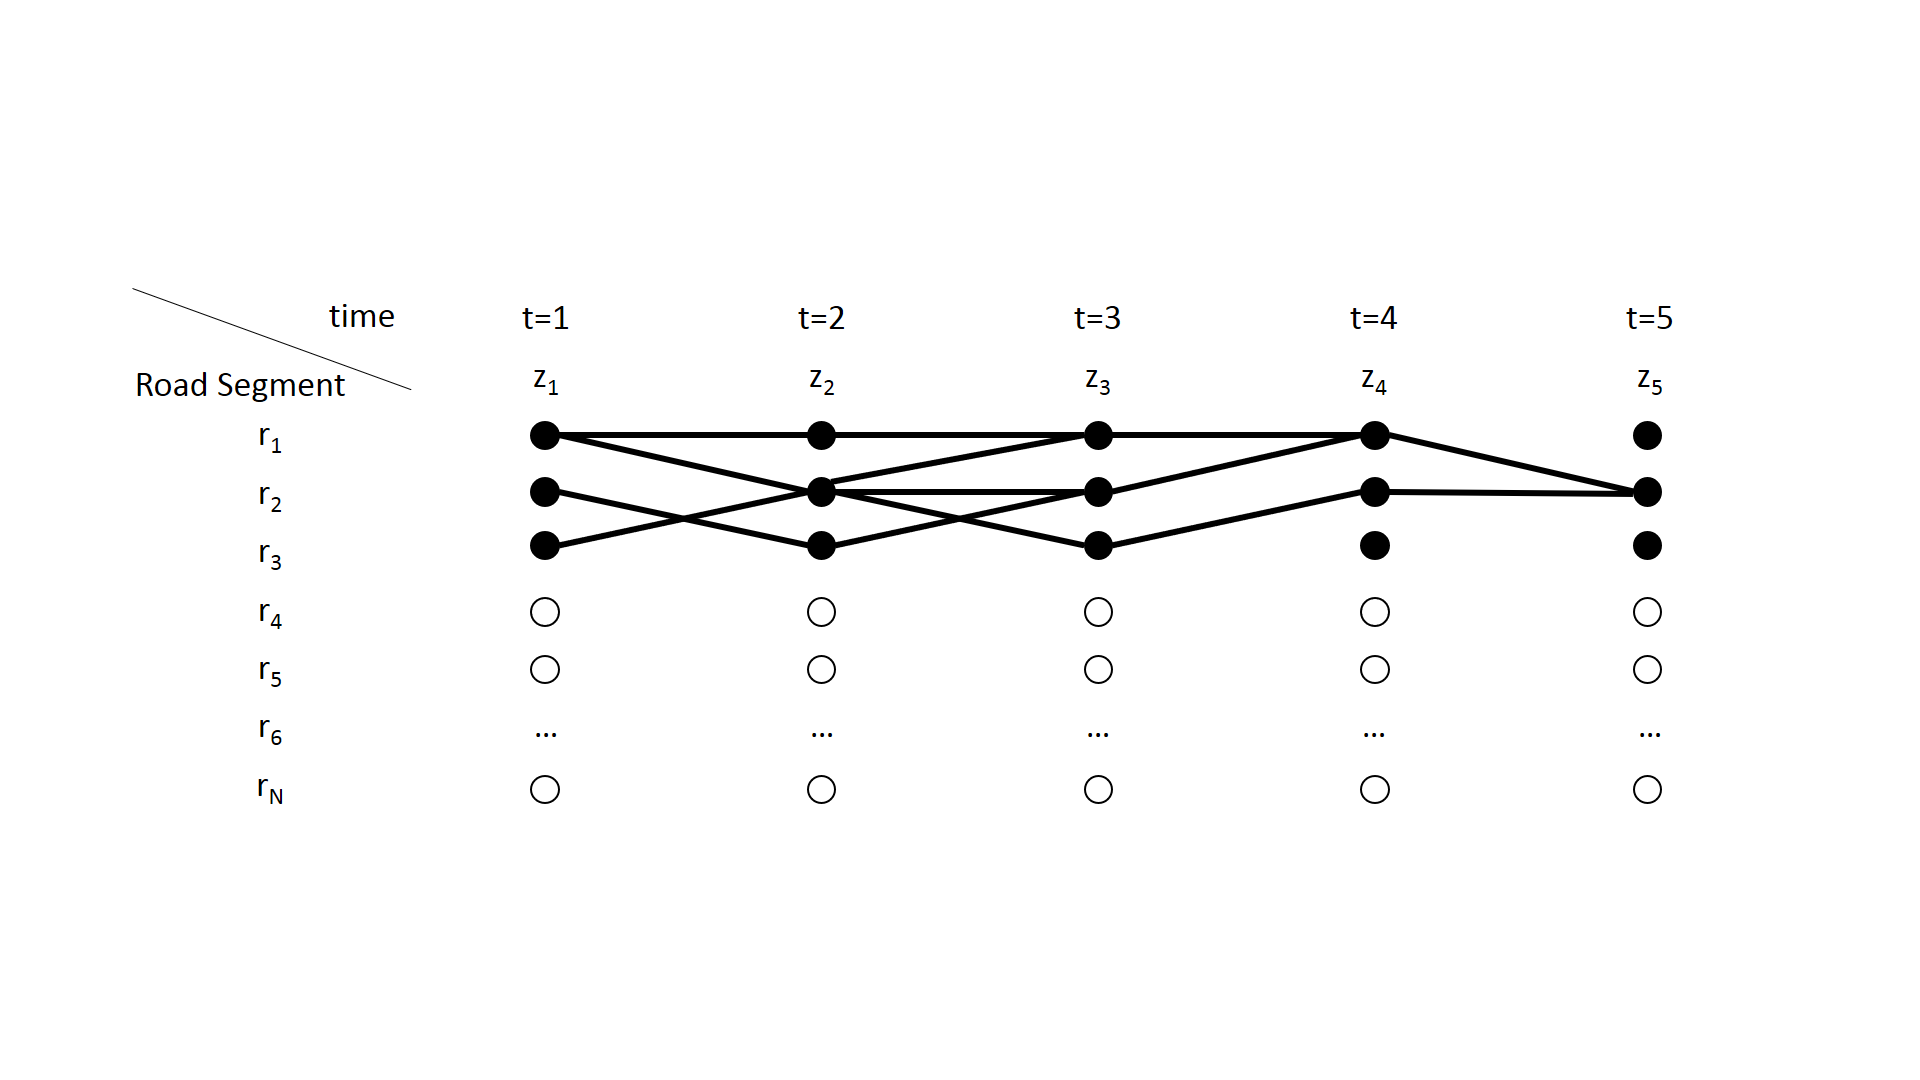
\includegraphics[width=1.0\textwidth]{fig2.png}
\caption{\label{fig:data} The map matching representation in HMM}
\end{figure}

Emission probability is expressing the probability of an observation being generated from a state. In this case, emission probability $p(z_t|r_i)$ gives the likelihood that the measurement $z_t$ would be observed if the vehicle were actually on road segment $r_i$ as depicted in Figure 3. Transition probability is representing the probability of moving from state $i$ to state $j$. In our map matching case, the transition probabilities $p(r_j|r_i)$ give the probability of a vehicle moving between the candidate road matches at these two times. 

\begin{figure}
\centering
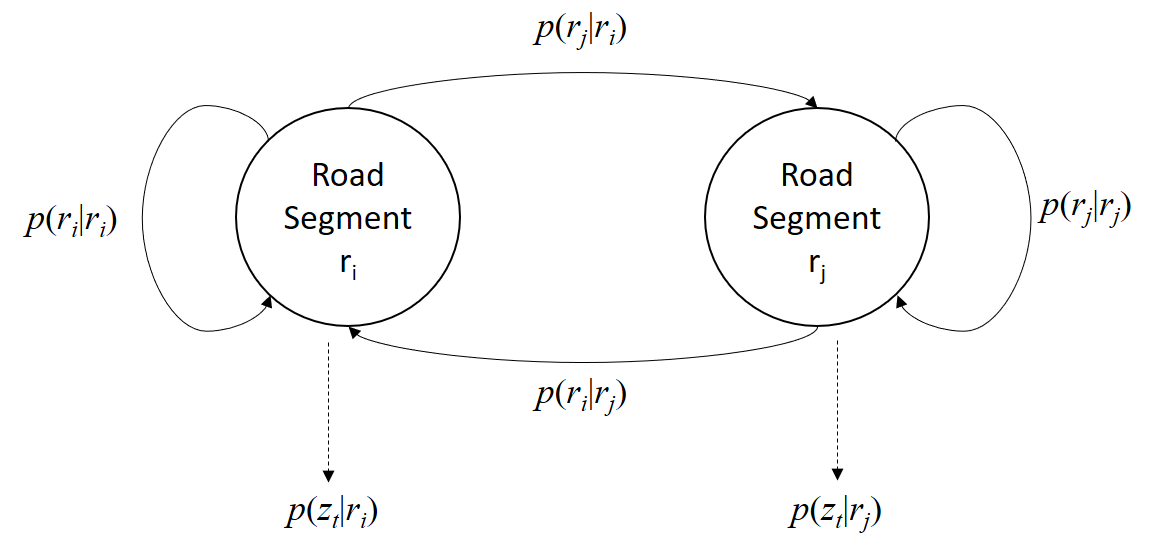
\includegraphics[width=1.0\textwidth]{fig3.png}
\caption{\label{fig:data} Transition and Emission Probabilities}
\end{figure}

For each input GPS position, a number of map matching candidates within a certain radius around the GPS position is computed. The Viterbi algorithm as provided by the hmm-lib is then used to compute the most likely sequence of map matching candidates. Thereby, the distances between GPS positions and map matching candidates as well as the routing distances between consecutive map matching candidates are taken into account. The GraphHopper y routing engine is used to find candidates and to compute routing distances.

The accuracy of map matching algorithm can be quantified by comparing the ground truth route to the route determined by the algorithm. Error measurement is illustrated in the Figure 4. Precisely, sum of the lengths of incorrect road added to and subtracted from the correct route. This sum is divided by the length of the correct route to compute the fraction of incorrect route. 

\begin{figure}
\centering
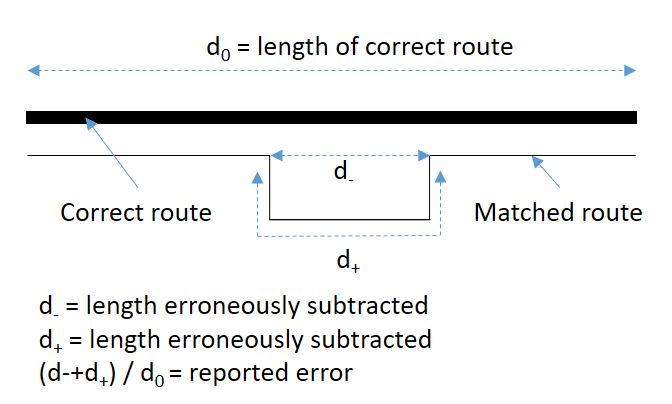
\includegraphics[width=1.0\textwidth]{fig4.png}
\caption{\label{fig:data} Error measurement}
\end{figure}

\section{Experiment and Discussion}
\label{sec:experiment}

Data is obtained from OpenStreetMap website [3], we use Leipzig city in Germany, since this city provides some trajectories data. GraphHopper API is used as routing engine to find candidates and to compute routing distances. The ground truth is road network that obtained from OpenStreetMap data.To assess the robustness of our HMM to matching the trajectory data with road network, we conduct an experiment with seven various type of trajectory data. The result is shown in figure 5 to 11. The black trace corresponds to trajectory data from GPS, the green trace represents the corrected trajectory data.

\begin{figure}
\centering
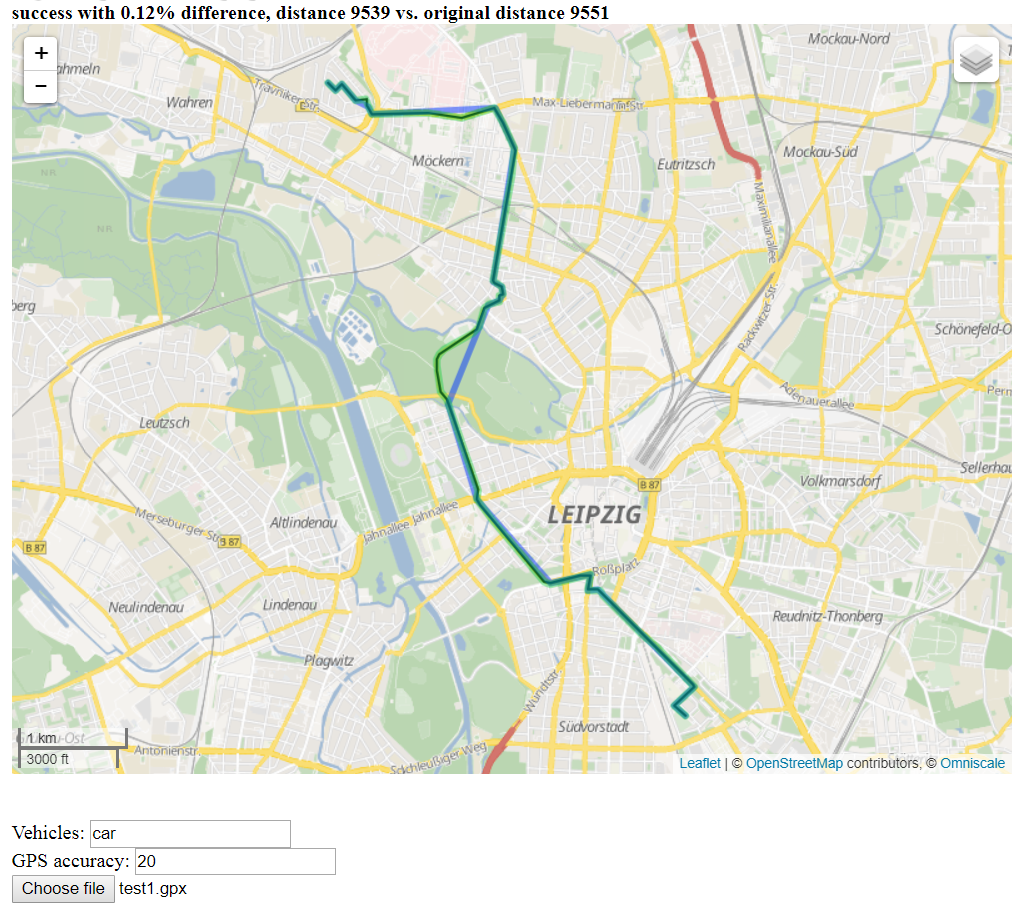
\includegraphics[width=0.75\textwidth]{fig5.png}
\caption{\label{fig:data} Test 1. Common car trajectory data }
\end{figure}

\begin{figure}
\centering
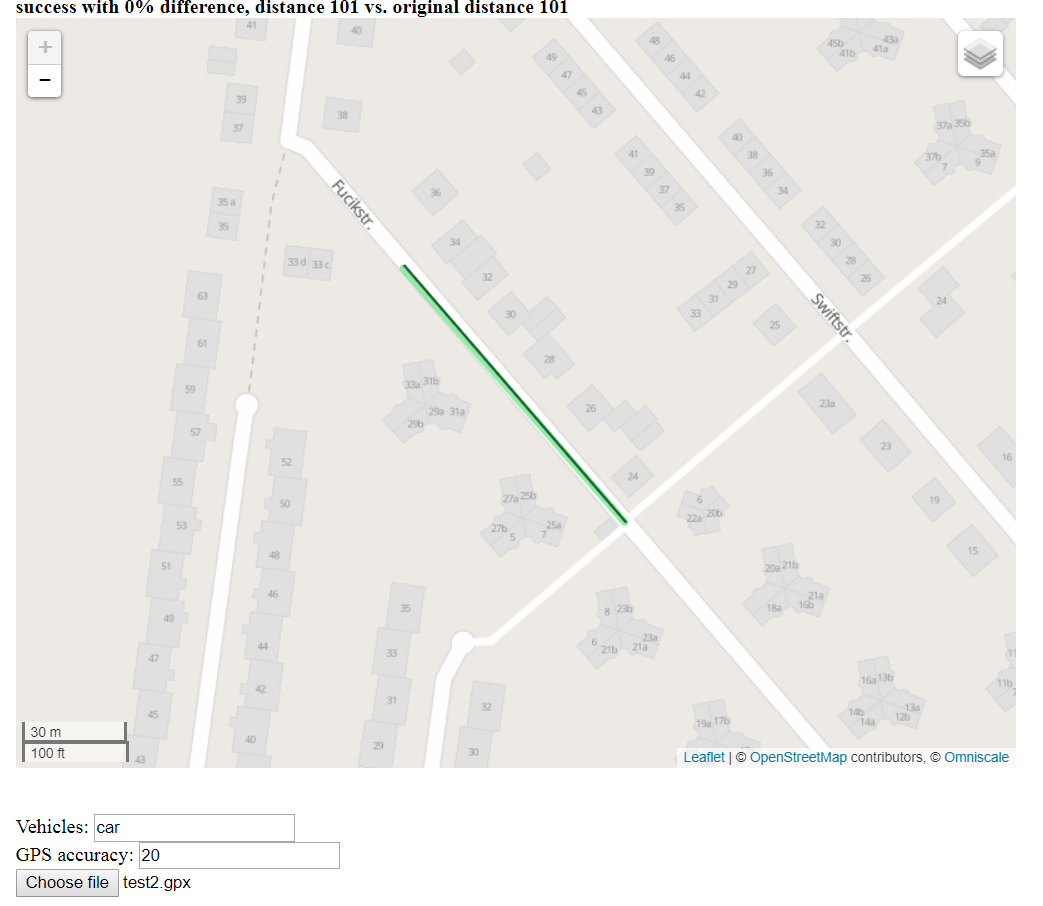
\includegraphics[width=0.75\textwidth]{fig6.png}
\caption{\label{fig:data} Test 2. A straight trajectory data }
\end{figure}

\begin{figure}
\centering
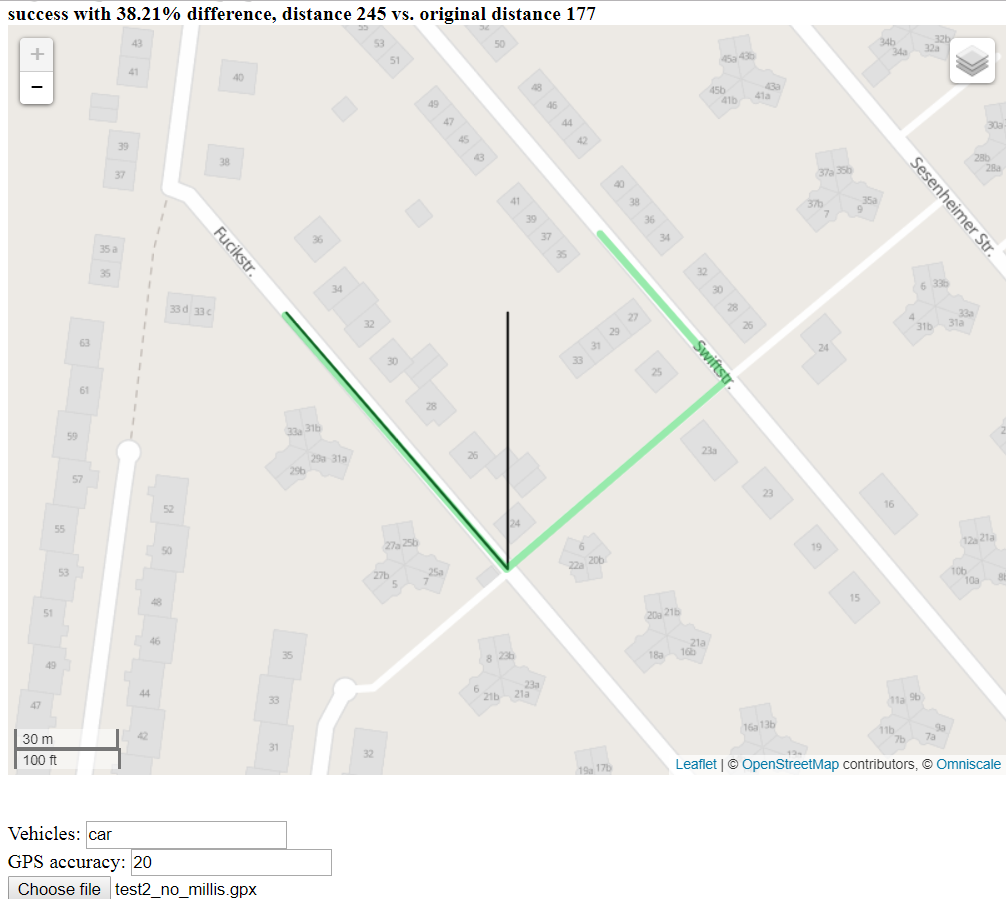
\includegraphics[width=0.75\textwidth]{fig7.png}
\caption{\label{fig:data} Test 3. Trajectory data with not end up on road network }
\end{figure}

\begin{figure}
\centering
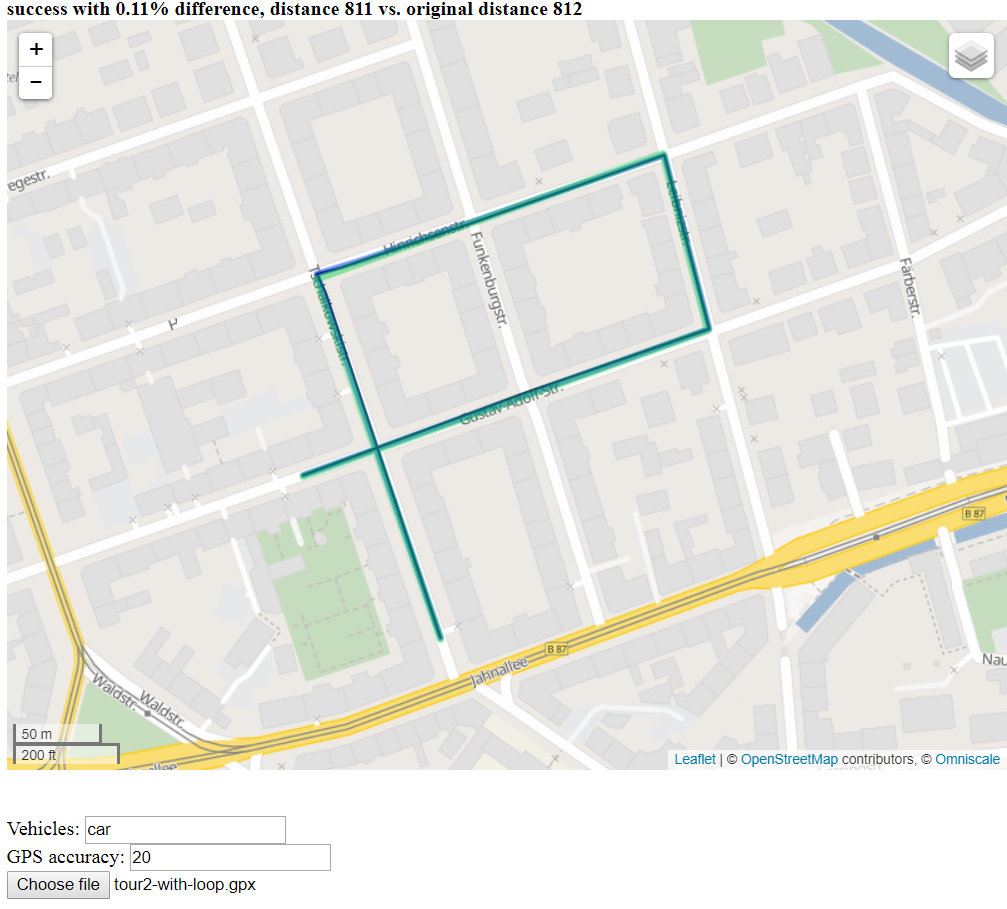
\includegraphics[width=0.75\textwidth]{fig8.png}
\caption{\label{fig:data} Test 4. Trajectory data with a loop }
\end{figure}

\begin{figure}
\centering
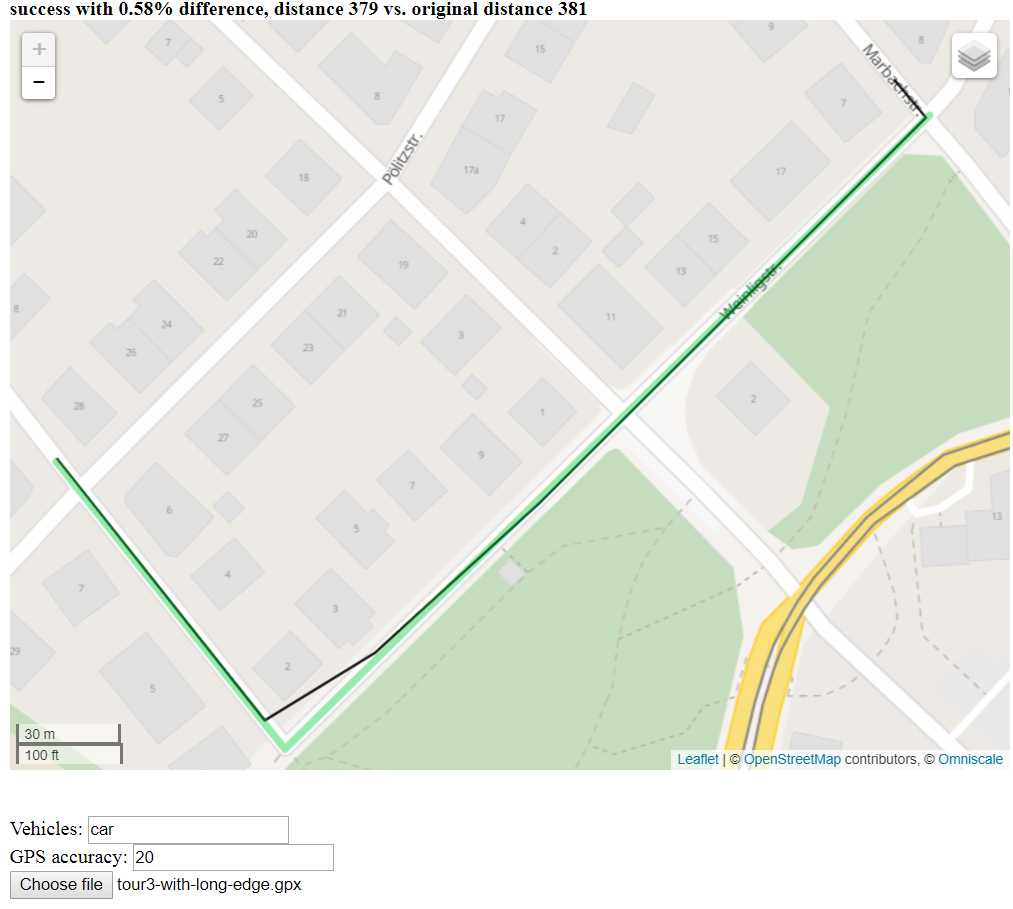
\includegraphics[width=0.75\textwidth]{fig9.png}
\caption{\label{fig:data} Test 5. Trajectory data with an error in long edge of road }
\end{figure}

\begin{figure}
\centering
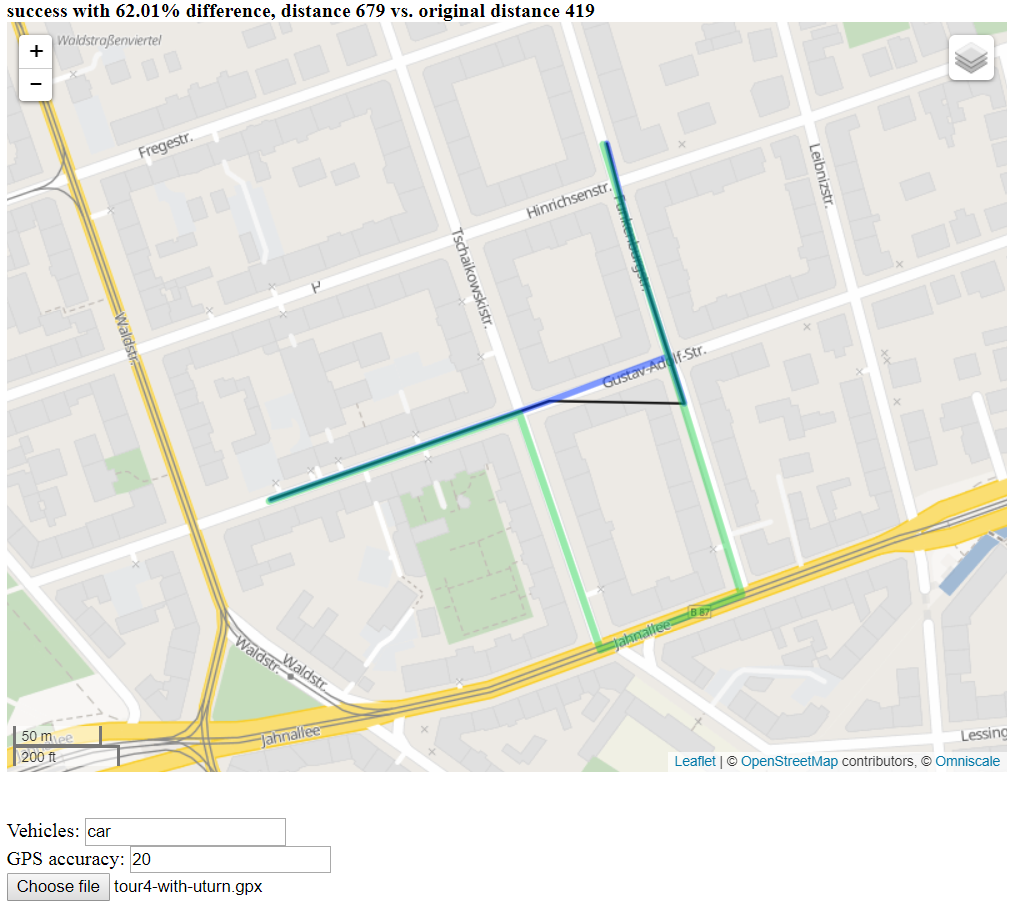
\includegraphics[width=0.75\textwidth]{fig10.png}
\caption{\label{fig:data} Test 6. Trajectory with error in U turn }
\end{figure}

\begin{figure}
\centering
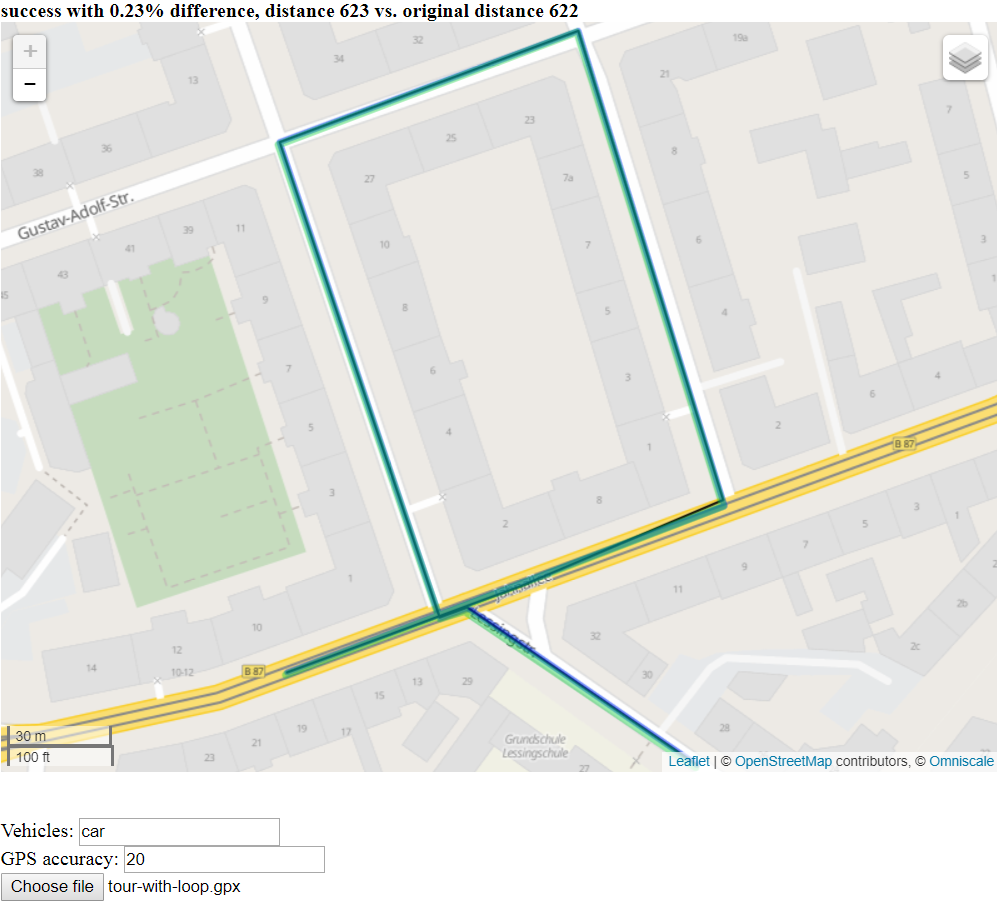
\includegraphics[width=0.75\textwidth]{fig11.png}
\caption{\label{fig:data} Test 7. Trajectory with an overlapping loop }
\end{figure}

\begin{table}[]
\centering
\begin{tabular}{|c|c|c|c|}
\hline
Data    & Error rate & Predicted distance & Actual distance \\ \hline
test 1  & 0.12       & 9539               & 9551            \\ \hline
test 2  & 0          & 101                & 101             \\ \hline
test 3  & 38.21      & 245                & 177             \\ \hline
test 4  & 0.11       & 811                & 812             \\ \hline
test 5  & 0.58       & 379                & 381             \\ \hline
test 6  & 62.01      & 679                & 419             \\ \hline
test 7  & 0.23       & 623                & 622             \\ \hline
Average & 14.46      &                    &                 \\ \hline
\end{tabular}
\caption{\label{fig:data} Summary of error rate and distance of predicted and actual trajectory }
\end{table}

The HMM model was working perfectly in data test 2, it is a straight trajectory, therefore HMM model does not encounter any difficulty in this trajectory data. While the high error happens in data test 3 and 6 having error rate 38.21 and 62.01, respectively. In data test 3, actual trace of GPS ends up to home, while the ground truth data (road-network) have not detail road until small road to the home. Furthermore, HMM model predict the longer distance compare with the distance of real trajectory data, due to the upper road is the nearest road to the last point of the trajectory. Test 6 data is a noisy trajectory with U turn pattern, the error rate is high due to the sampling time of trajectory is high, it goes to different road before it turns to destination road. Overall the error rate of our HMM model is 14.46, this result is quite satisfaction for the initial research to map matching vehicle to the road network.

\section{Conclusion and Futurework}
\label{sec:conclusion}

We proposed Hidden Markov Model to tackle map matching problem in road network trajectory. By using Viterbi algorithm, we can obtain the most likely road network which fit with the input trace data. Our HMM model obtained a good result, except in U turn trace problem as shown in figure 8 having error rate more than 50\%, and trajectory data that end up in particular place that having no road network in the ground truth data (figure 5).

In future work, to reduce the error rate, we plan to use more fine-grained technique, such as adding similarity measure algorithm in matching the most likely road candidate with input trace data.


\begin{thebibliography}{9}
\bibitem{nano3}
Newson, Paul, and John Krumm. "Hidden Markov map matching through noise and sparseness." Proceedings of the 17th ACM SIGSPATIAL International Conference on Advances in Geographic Information Systems. ACM, 2009.
\bibitem{nano3}
https://www.graphhopper.com/ 
\bibitem{nano3}
https://www.openstreetmap.org/ 
\bibitem{nano3}
Guanfeng Wang and Roger Zimmermann. “An Error-bounded Delay-bounded Real-time Map Matching Algorithm using HMM and Online Viterbi Decoder”. Proceedings of the 22nd ACM SIGSPATIAL International Conference on Advances in Geographic Information Systems. ACM, 2014.
\bibitem{nano3}
Takayuki Osogami and Rudy Raymond. “Map Matching with Inverse Reinforcement Learning”. IJCAI. 2013.
\end{thebibliography}
\end{document}